\pdfoutput=1

\documentclass{l4proj}

%
% put any packages here
%
\usepackage{float}

\begin{document}
\title{On The Scalability of ROS}
\author{Isaac Jordan}
\date{\today}
\maketitle

\begin{abstract}
Robots, distributed systems, and middleware.
\end{abstract}

\educationalconsent
%
%NOTE: if you include the educationalconsent (above) and your project is graded an A then
%      it may be entered in the CS Hall of Fame
%
\tableofcontents
%==============================================================================

\chapter{Introduction}
\pagenumbering{arabic}

\section{Context}

Robotics is the field of creating physical systems to automate tasks. As a concept, automation dates back hundreds of years - however the idea of replicating biological systems seen in nature (for example, humans) was not first seen until the 20th century. Robotics was mainly considered a theoretical or fictitious fantasy, however the main discussers of the concept (such as Isaac Asimov) assumed technological capability would inevitably reach the level where robotics would either be inseperable from society, or be banned due to it's impact.

In the 19th century the beginnings of robotics could be seen in the creation of vehicles which could be remotely operated using electric signals. By the early 20th century, wireless radio guidance systems were advanced enough that remotely operated aircraft could be demonstrated in 1917 (by Archibald Low [citation needed]).

Technology advanced so rapidly during the 20th century that by the 1970s the Soviet Union could explore the surface of the moon using a remotely operated vehicle robot.

However, these uses of robotics displayed no `intelligent behaviour' on behalf of the robotic system. Beginning in the 1980s, the growing field of Artificial Intelligence (A.I.) was revived and began creating systems which could intelligently answer domain-specific questions - called expert systems. 

Robotics is a fast-progressing field which has seen major advances the past decades. From obvious examples such as Amazon's item pickers, to more integrated applications such as autonomous cars - the scale of robotics is increasing.

\section{Aims and Objectives}

If I had an aim it would go here.

\section{Achievements}

If I had achieved anything it would go here.



%\vspace{-7mm}
%\begin{figure}
%\centering
%\includegraphics[height=9.2cm,width=13.2cm]{uroboros.pdf}
%\vspace{-30mm}
%\caption{An alternative hierarchy of the algorithms.}
%\label{uroborus}
%\end{figure}

\chapter{Background}

\section{Robotics}

Robots are the future. (Why robots are important)

Robotics is the field concerning autonomous computer systems, usually involving physical interaction with it's environment. Robotics lies at the intersection between computing science, eletrical and mechanical engineering. Robotics has been common in popular culture since the 1940s, however the physical realisation of these systems did not begin to be practical until the 2000s when increases in computing power, sensor accuracy, research investment, and software algorithms allowed for useful robotics systems to be created.

Today's robotic systems generally consist of many small autonomous systems working together to form a coherent whole. For example, a particular sensor (say a camera) may be constantly recording data and storing it in some buffer (erasing the oldest when full). This subsystem does not depend on any others to complete it's task (recording the envionrment), but other subsystems may rely on it's output (such as a computer vision package which needs video frame inputs).

\section{Multi-Robot Systems}

Multi-robot systems are specific instances of mult-agent systems. They represent a joint problem space between robotics, artificial intelligence, and distributed systems. Multi-robot systems as a formal concept is a recent development with a IEEE technical committee only being formed in 2014\cite{MultiRobotSystemsIEEECommittee}.

Multi-robot systems can consist of many intelligent agents (each of which may be comprised of many small autonomous systems) working to solve a task that any one system may not be able to solve alone. One such example is a warehouse management system. 

In a warehouse, millions of items can be spread throughout miles of shelving and the requirement is that a random subset of items (those that have been bought) must arrive at a specific point (the delivery pick-up point) at a specific time (when the van is there). This task previously could be solved by having human pickers wander the isles searching for items - however given recent increases in the size of online shopping this is no longer feasible. Now, online retailers are using thousands of individual robots to intelligently move the shelving around and bring the correct items to stationary human pickers. This system requires the coordination of the individual robots, but they must all act independently in order to efficiently keep pace with the items ordered.

\section{Scalability in Robotics}

When creating multi-robot systems, scalability becomes an important concern. At what level does a system architect choose to switch from small highly-powered robot systems to a larger number of simpler robot systems. Several factors to consider include the processing power of each robot, the communication framework required to organise them, the cost of each robot, and the suitability of the problem to a multi-robot system.

Swarm robotics is the extreme approach of creating many very simple robots which individually could not solve tasks or survive environments - however when they work together as a form of society they can work efficiently.

\section{Robotic Middleware}

Robot designers want to work at a high level. Sensors are low level. (Why is middleware needed, whats available)

Robotic middleware is a software infrastructure that is intended to provide convenient abstraction and communication paradigms for facilitating this multi-subsystem approach. In general, a robotics middleware would provide interfaces for defining each subsystem, and defning how each subsystem communicates with others.

Insert middlware overview here!

\section{ROS (Robot Operating System)}

ROS is what I'll be testing out. (What is it)

\section{Configuration of Robots}

The robots used in this project are 9 identical robot cars with front-wheel steering. (What is their set up)


\chapter{Experimental Analysis}

\section{Experiment 1}

The first experiment was designed to analyse the transfer time of messages between two machines at varying message frequencies. This would highlight whether there was some limit as to how often ROS could send and receive messages on it's topics.

\subsection{Configuration}

These two machines were Raspberry Pi 3 Model Bs connected via ethernet to an Asus router.

The messages were sent and received using ROS Kinetic, running on the Raspbian OS.

The experimental setup was that one Raspberry Pi would run a ROS master node, another Raspberry Pi runs a sender program that notes down the message-sent time, and sends it to a 3rd Raspberry Pi which merely echoes the message back to the sender. Upon receiving the message, the sender/receiver notes the current time, and writes `message X which was sent at Y, was received at Z' to a text file. The resulting Round Trip Time (RTT) for each message would therefore be the difference between the message-sent time and the message-received time.

The expected result of the experiment was that message latency (RTT) would be the same across all lower frequencies, until some bottleneck was reached that would then cause message latencies to exponentially increase due to congestion.

Code had been written prior to execute this experiment, so initially this was used\cite{Experiment1InitialCode}. However, this gave results that were contrary to the hypothesis. An increase in message frequency resulted in a reduction in message latency. A number of messages on higher frequencies were also dropped, and never received. As this was the opposite of the hypothesis, the first step was to critique the experiment code.

This review highlighted two major issues, the first was the echoing machine had a delay similar to the sender when the experiment design mandated that the echoer always respond as fast as it can. The second issue was the the maximum message queue size in ROS (how many messages can be buffered at once to compensate for a slow subscriber) was set equal to the message frequency of that run.

These issues were resolved by removing the code that executed the delay in the echoer, and by setting the maximum queue size to be equal to 1000 in every experiment (the number of messages expected to be sent).

The experiment was then repeated using this code, and the results from these runs agreed with the hypothesis.

\section{Experiment 2}

Experiment 2 was an investigation in to whether the performance of ROS messages was affected by previous messages sent on the system. This was tested by comparing the performance of ROS messages of 5 consecutive message passing runs vs 5 message passing runs with system reboots between runs. This was repeated at 1KHz, 4KHz, 7KHz, and 10Khz frequencies for two reasons. The first was to investigate whether areas in which we observed consistent performance before would exhibit any difference between reboot and no reboot. Secondly, it would give further insight in to where the exact barrier between `good, consistent performance' and `poor, erratic performance' is.

Rebooting the systems involved has the opportunity to affect performance by stopping any background processes, interrupting slow processing messages from previous runs, and resetting any message caches and buffers in memory.

The result of the experiment was hypothesised to demonstrate no significant difference between rebooting and not-rebooting at any message frequency.

\begin{figure}[h]
\centering
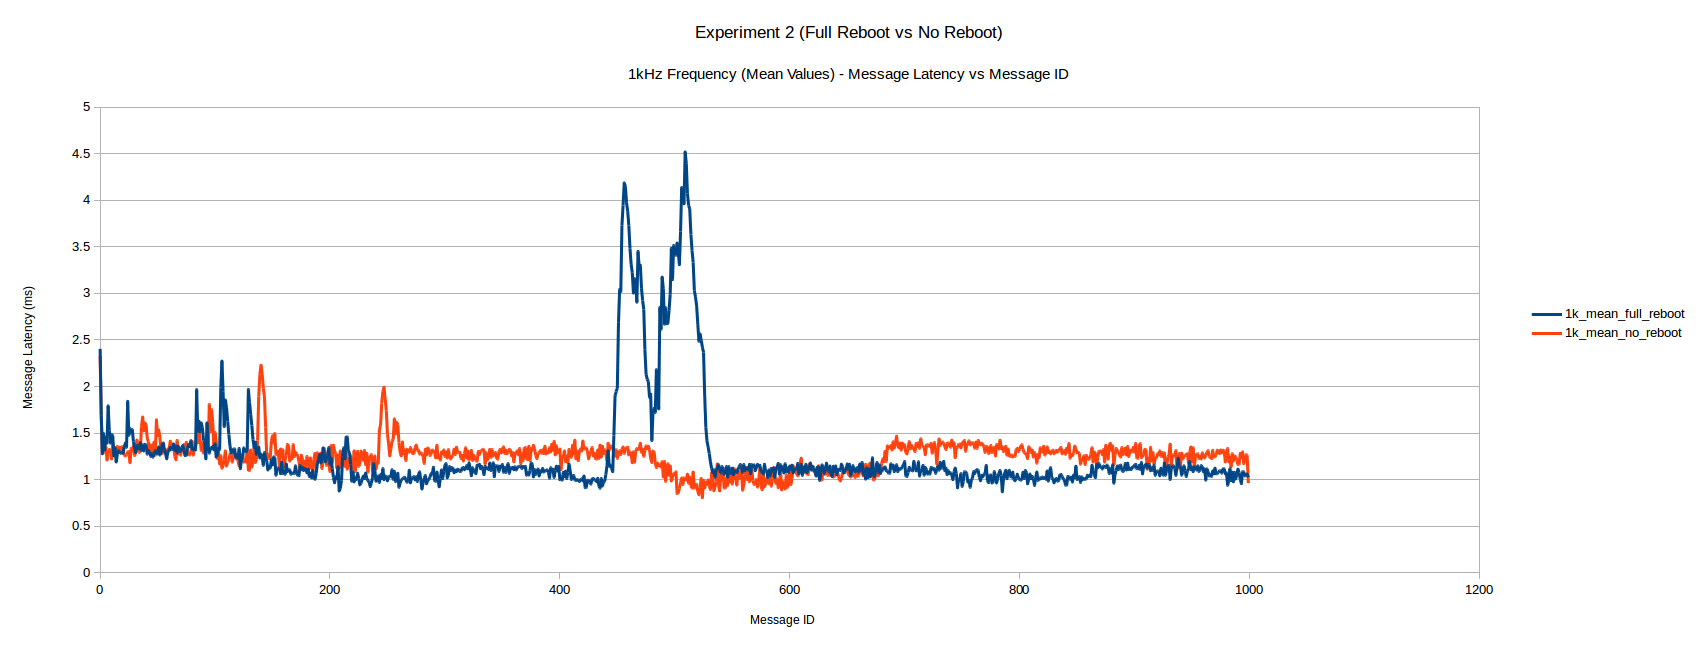
\includegraphics[width=\textwidth]{images/1khz-mean.png}
\caption{Experiment 2 - Mean Message Latency 1KHz Message Frequency}
\label{exp2-1khz-mean}
\end{figure}

Figure \ref{exp2-1khz-mean} demonstrates that for relatively low message frequencies the mean message latency was consistently 1 - 1.5ms (the peak around message 500 in the full reboot data was due to 1 erroneous run at that data point). Figure \ref{exp2-4khz-mean} is characteristic of the higher frequency runs - the no reboot runs generally gave equal or better performance compared to the full reboot runs. See Appendix \ref{exp2-appendix-results} for other mean graphs, and individual run graphs.

\begin{figure}[h]
\centering
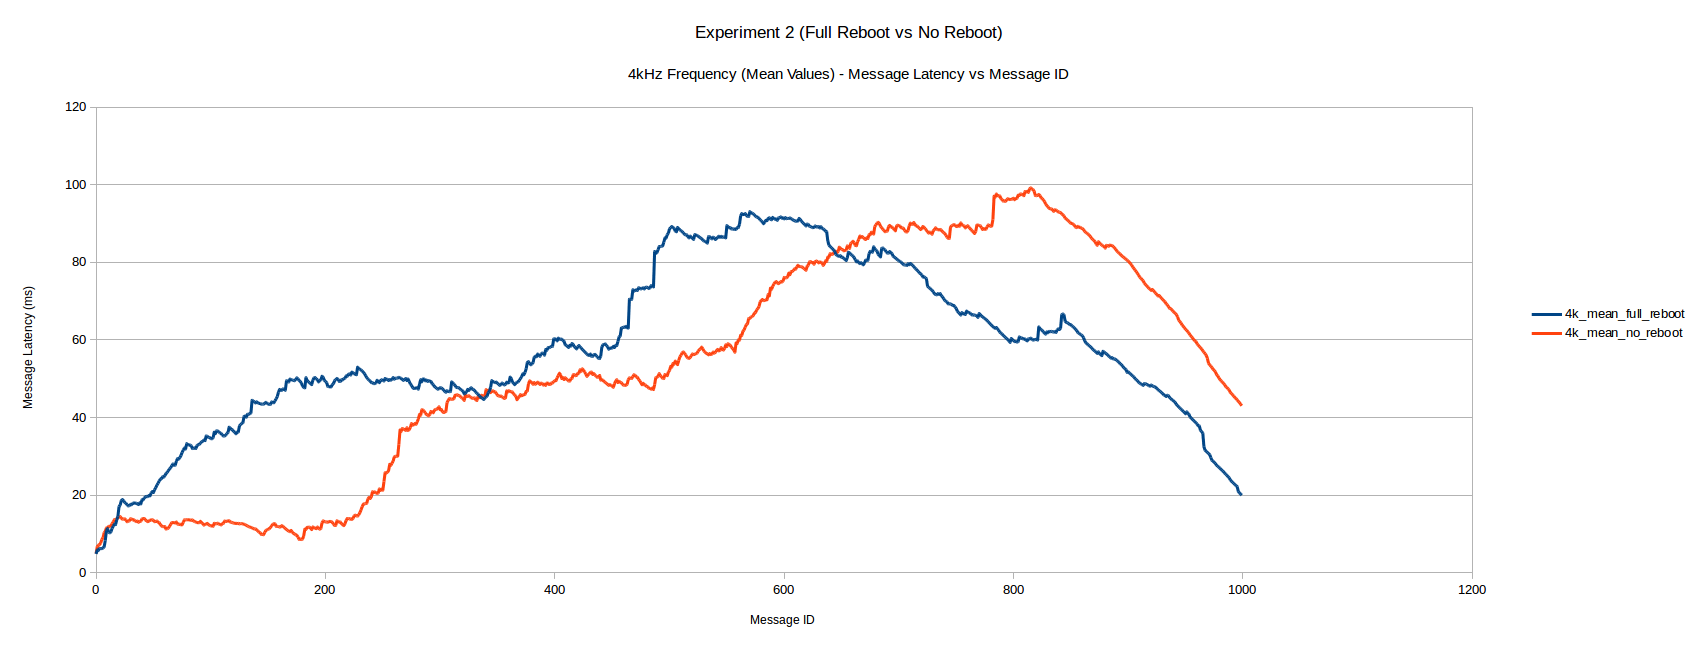
\includegraphics[width=\textwidth]{images/4khz-mean.png}
\caption{Experiment 2 - Mean Message Latency 4KHz Message Frequency}
\label{exp2-4khz-mean}
\end{figure}

%%%%%%%%%%%%%%%%
%              %
%  APPENDICES  %
%              %
%%%%%%%%%%%%%%%%
\begin{appendices}

\chapter{Experiment 2 Other Graphs}
\label{exp2-appendix-results}

\begin{figure}
\centering
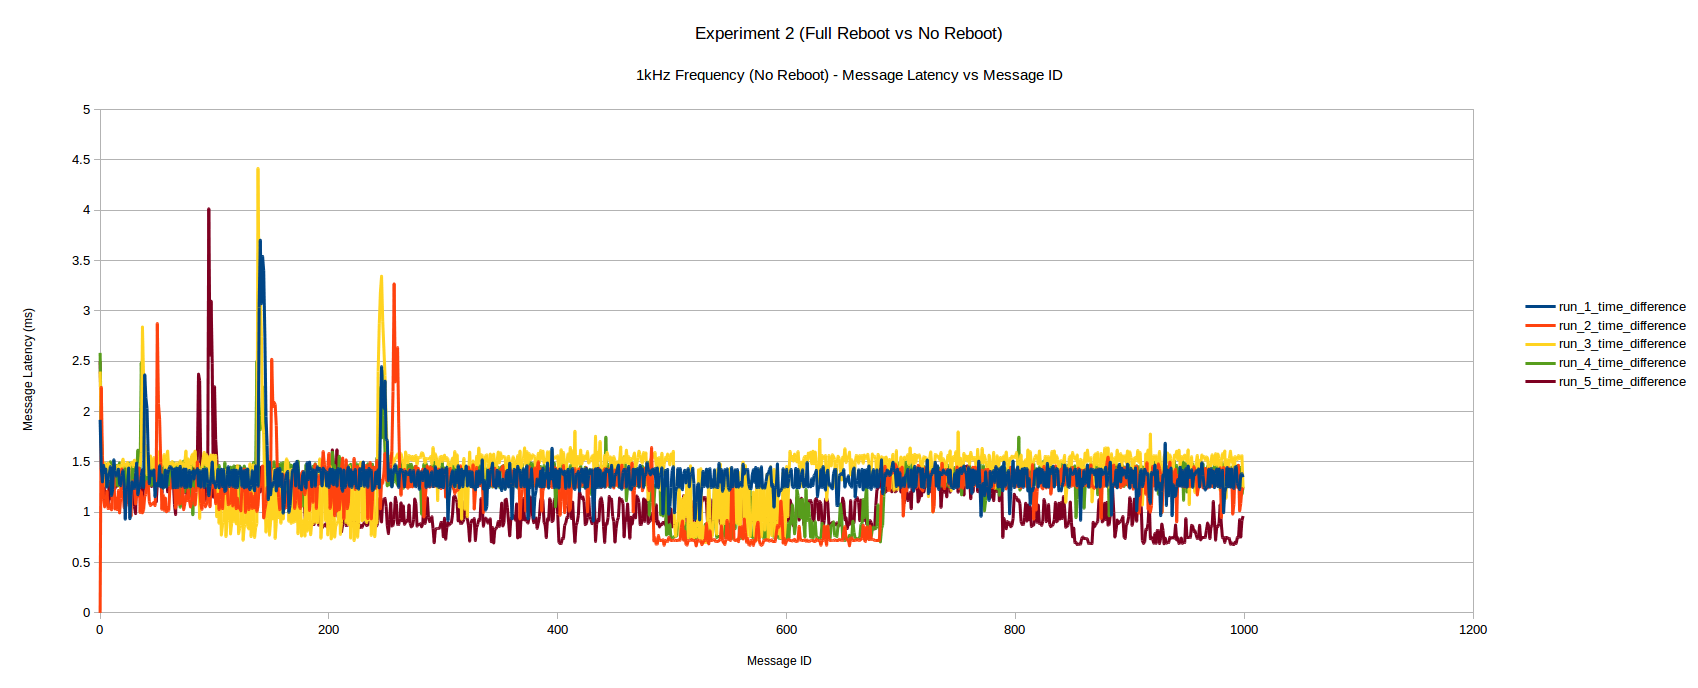
\includegraphics[width=\textwidth]{images/no-reboot-1khz.png}
\caption{Experiment 2 - No Reboot 1KHz Message Frequency}
\label{exp2-noreboot-1khz}
\end{figure}

\begin{figure}
\centering
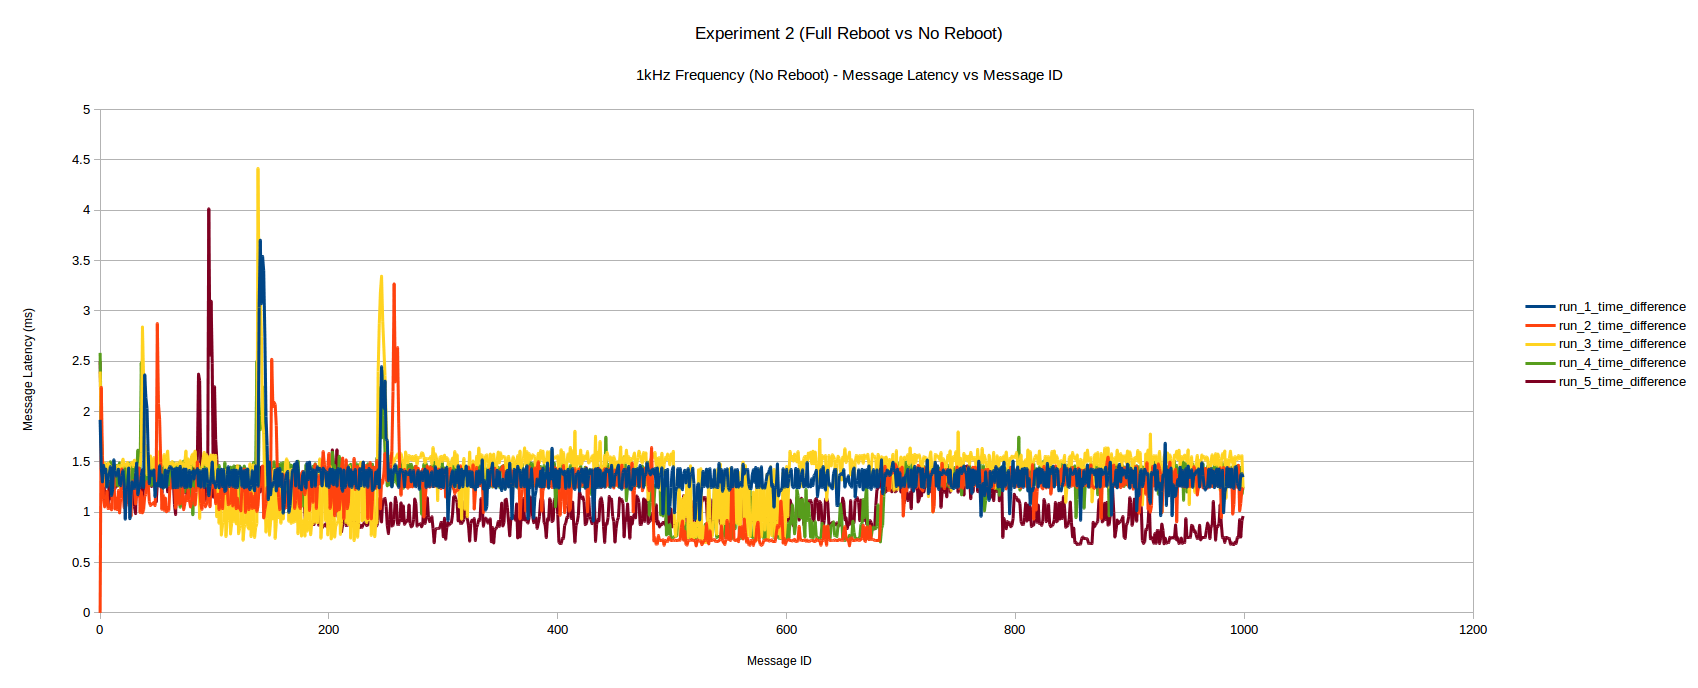
\includegraphics[width=\textwidth]{images/no-reboot-1khz.png}
\caption{Experiment 2 - No Reboot 1KHz Message Frequency}
\label{exp2-fullreboot-1khz}
\end{figure}

\begin{figure}
\centering
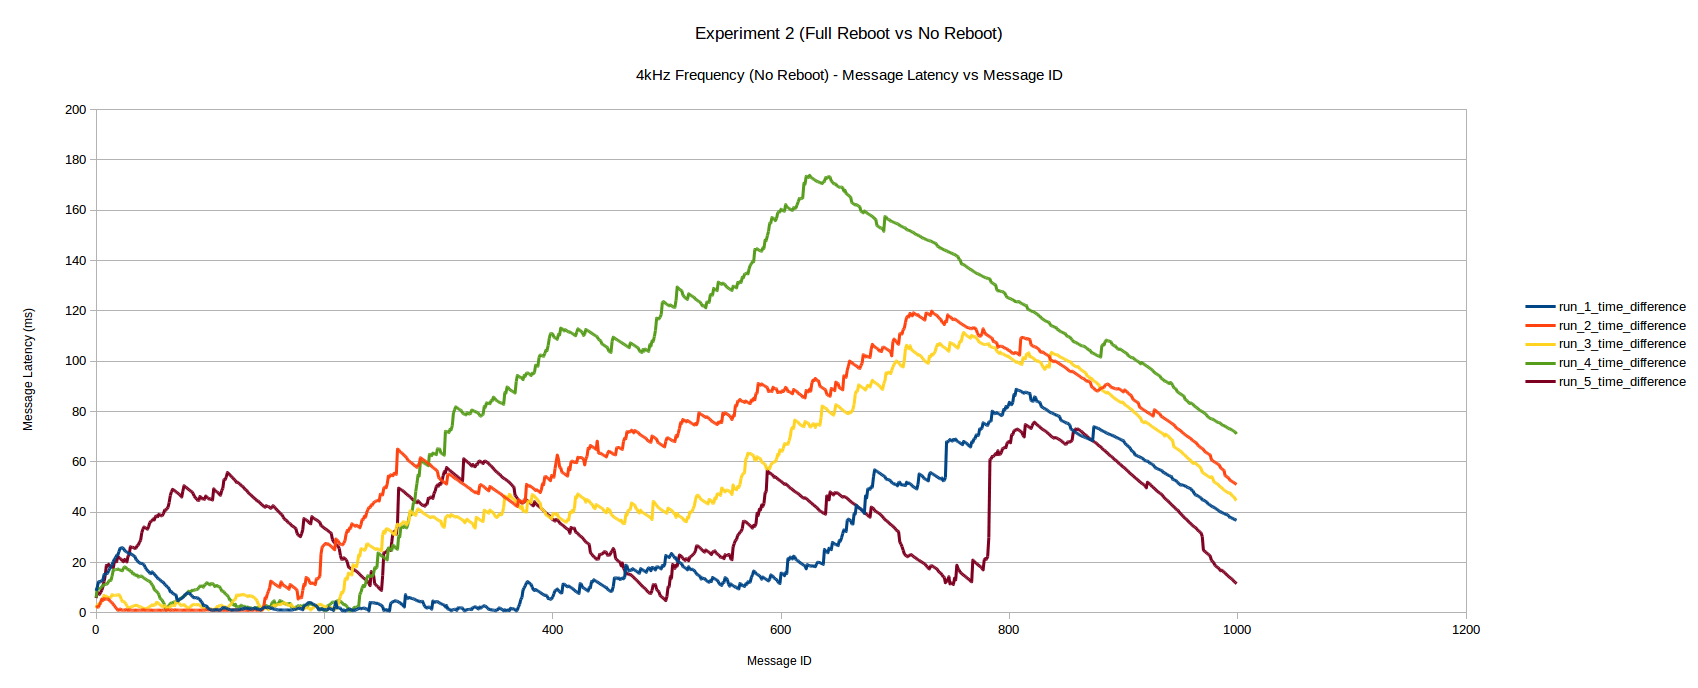
\includegraphics[width=\textwidth]{images/no-reboot-4khz.png}
\caption{Experiment 2 - No Reboot 4KHz Message Frequency}
\label{exp2-noreboot-4khz}
\end{figure}

\begin{figure}
\centering
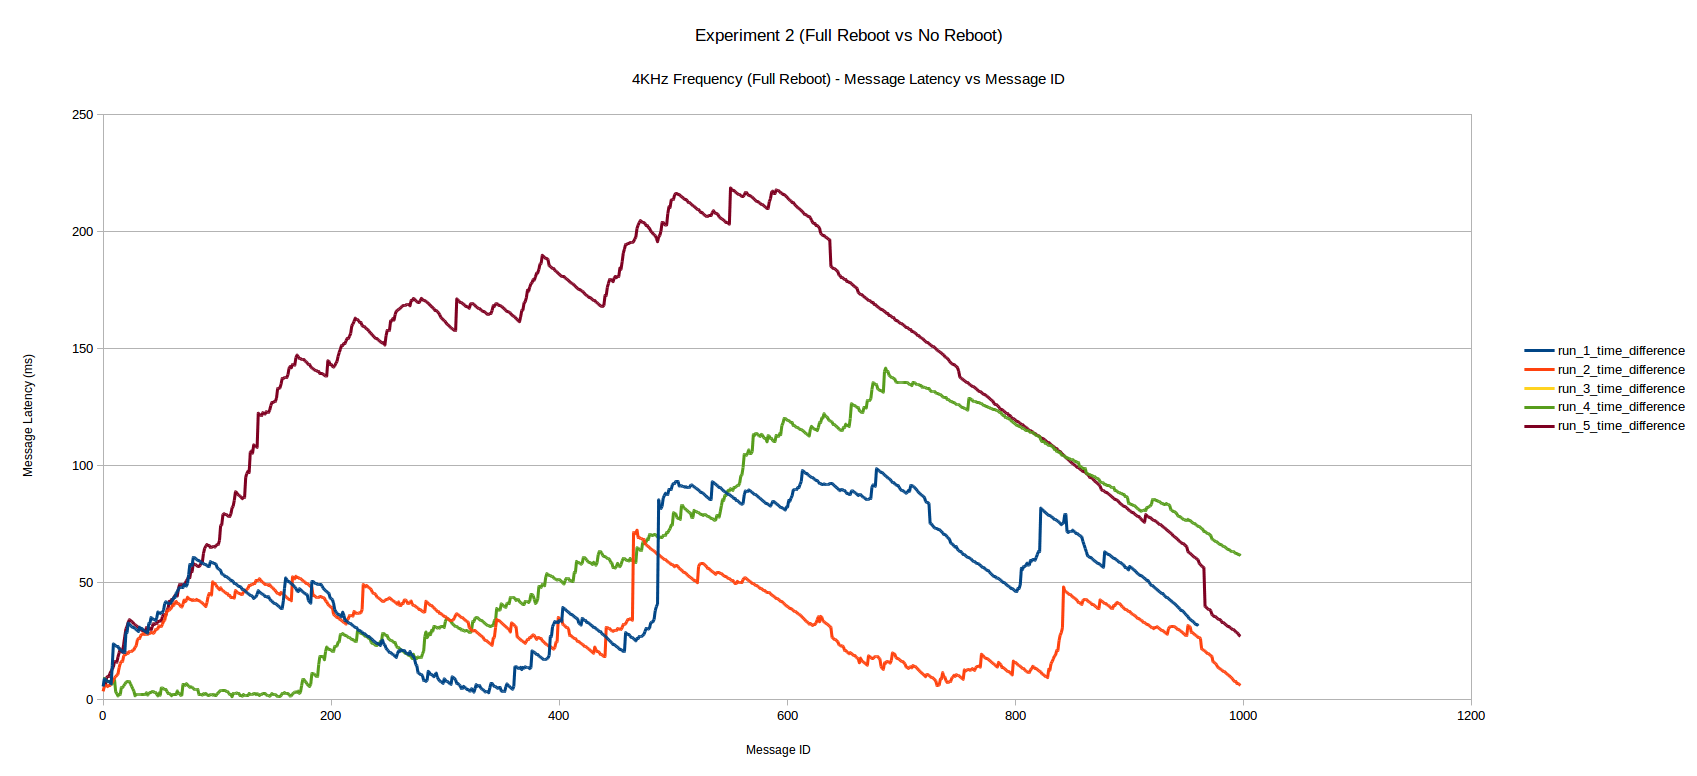
\includegraphics[width=\textwidth]{images/full-reboot-4khz.png}
\caption{Experiment 2 - Full Reboot 4KHz Message Frequency}
\label{exp2-fullreboot-4khz}
\end{figure}

\begin{figure}
\centering
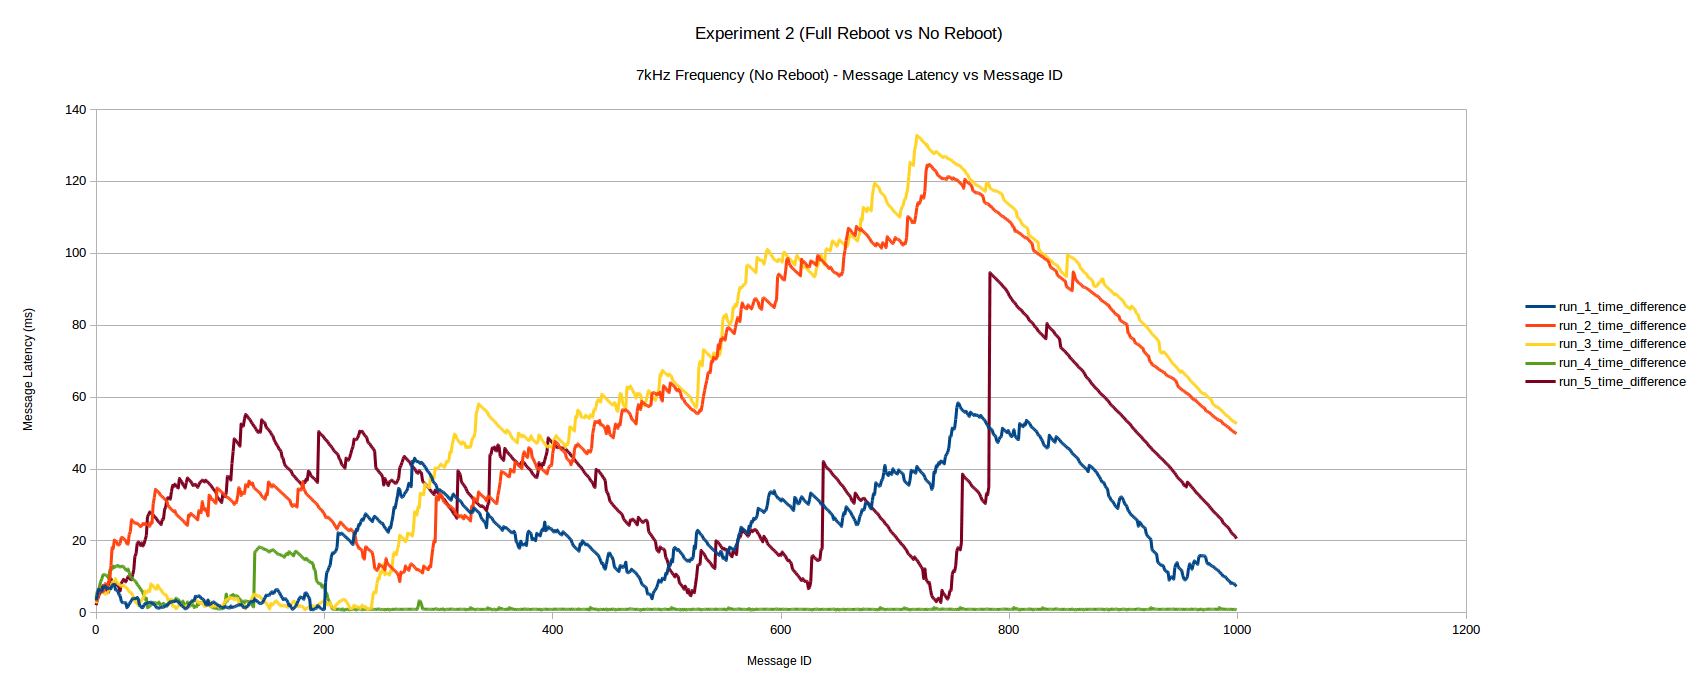
\includegraphics[width=\textwidth]{images/no-reboot-7khz.png}
\caption{Experiment 2 - No Reboot 7KHz Message Frequency}
\label{exp2-noreboot-7khz}
\end{figure}

\begin{figure}
\centering
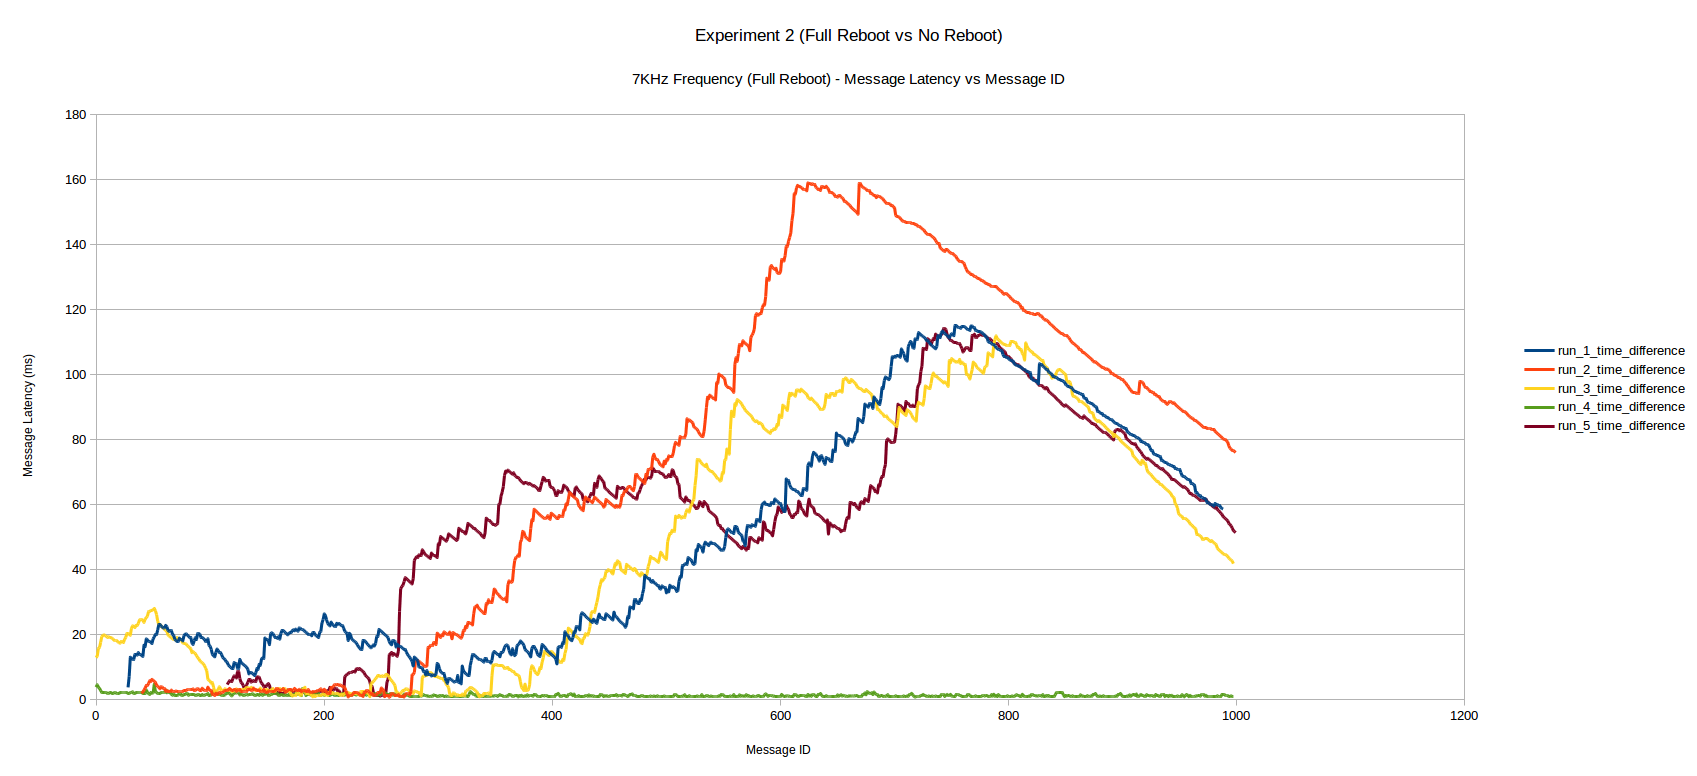
\includegraphics[width=\textwidth]{images/full-reboot-7khz.png}
\caption{Experiment 2 - Full Reboot 7KHz Message Frequency}
\label{exp2-fullreboot-7khz}
\end{figure}

\begin{figure}
\centering
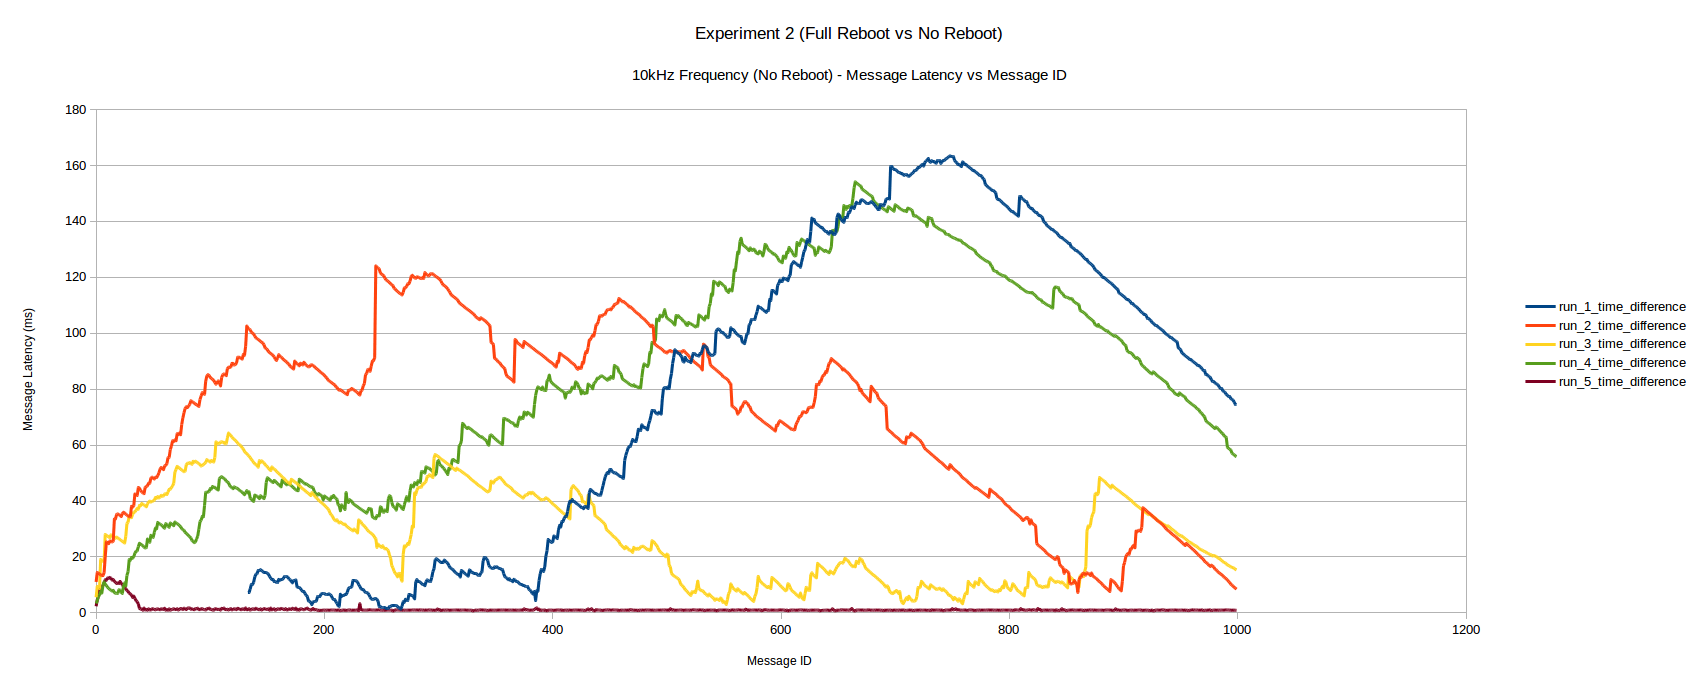
\includegraphics[width=\textwidth]{images/no-reboot-10khz.png}
\caption{Experiment 2 - No Reboot 10KHz Message Frequency}
\label{exp2-noreboot-10khz}
\end{figure}

\begin{figure}
\centering
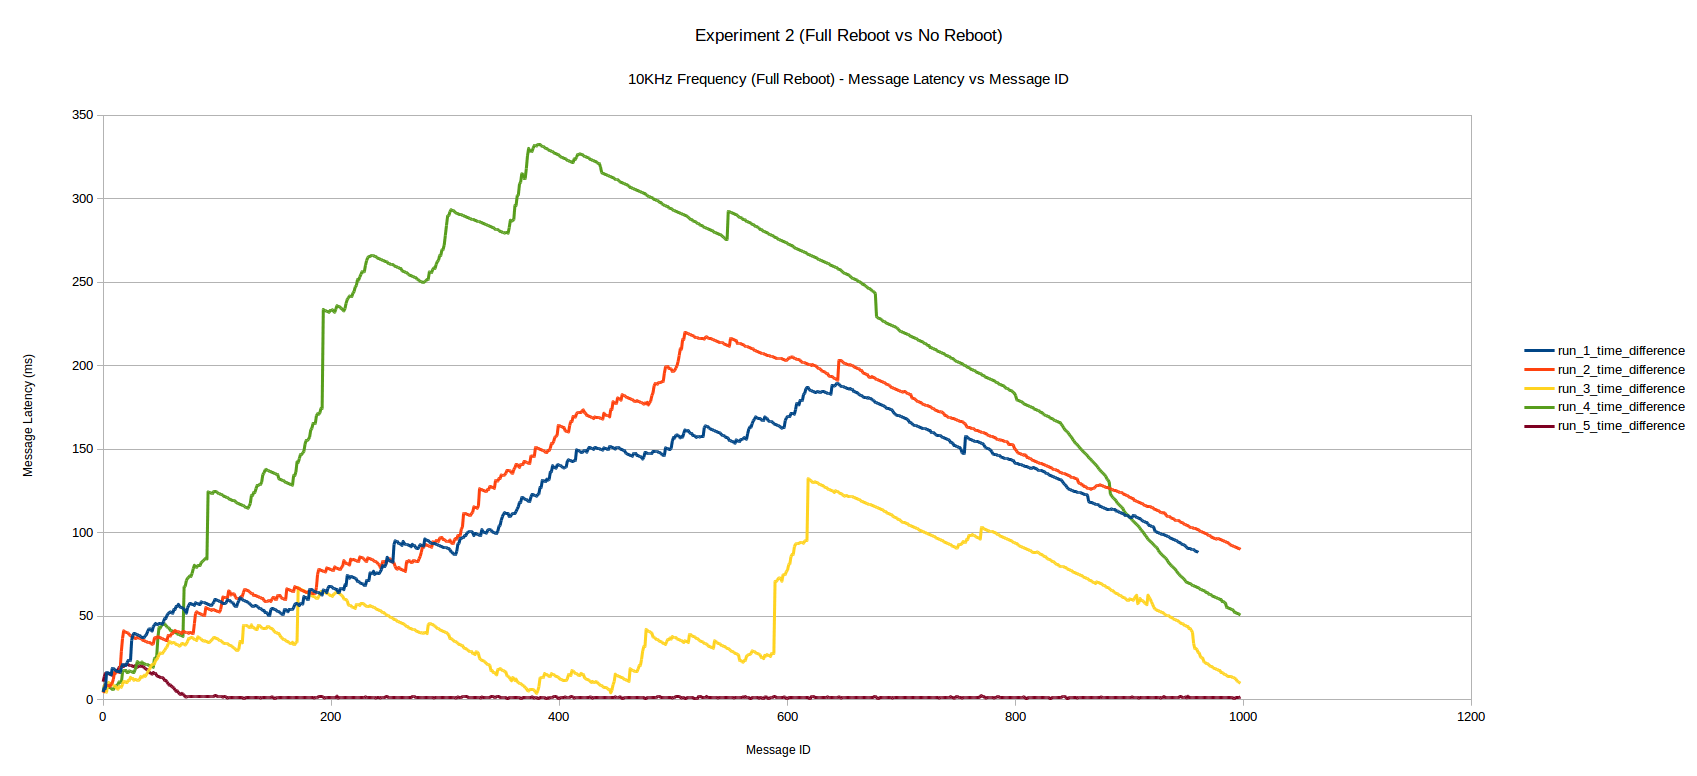
\includegraphics[width=\textwidth]{images/full-reboot-10khz.png}
\caption{Experiment 2 - Full Reboot 10KHz Message Frequency}
\label{exp2-fullreboot-10khz}
\end{figure}

\chapter{Running the Programs}

To compile this dissertation:
\begin{verbatim}

	> pdflatex dissertation
	> bibtex dissertation
	> pdflatex dissertation
    > pdflatex dissertation

\end{verbatim}


An example of running from the command line is as follows:
\begin{verbatim}
	> rosrun rosberry_experiments run_experiment.py
\end{verbatim}


\chapter{Generating Random Graphs (Example Appendix)}
\label{sec:randomGraph}

\begin{verbatim}
	> java RandomGraph 100 0.9 > 100-90-00.clq
\end{verbatim}
\end{appendices}

%%%%%%%%%%%%%%%%%%%%
%   BIBLIOGRAPHY   %
%%%%%%%%%%%%%%%%%%%%

\bibliographystyle{plain}
\bibliography{bib}

\end{document}
